\documentclass[11pt, a4paper]{article}
\usepackage[utf8]{inputenc}
\usepackage{geometry}
\usepackage{hyperref}
\usepackage{listings}
\usepackage{graphicx}
\graphicspath{ {./images/} }

\usepackage{biblatex}
\addbibresource{sources.bib}


\title{Simulazione delle Dinamiche Molecolari con CUDA\\ 
       \Large Resoconto finale}
\author{Enrico Verdolotti}
\date{Gennaio/Febbraio 2020}

\setlength{\parindent}{1em}
\setlength{\parskip}{1em}
\geometry{margin=2cm, top=2cm, bottom=2cm}
\pagenumbering{gobble}

\begin{document}

\maketitle


\begin{figure}[h]
\centering
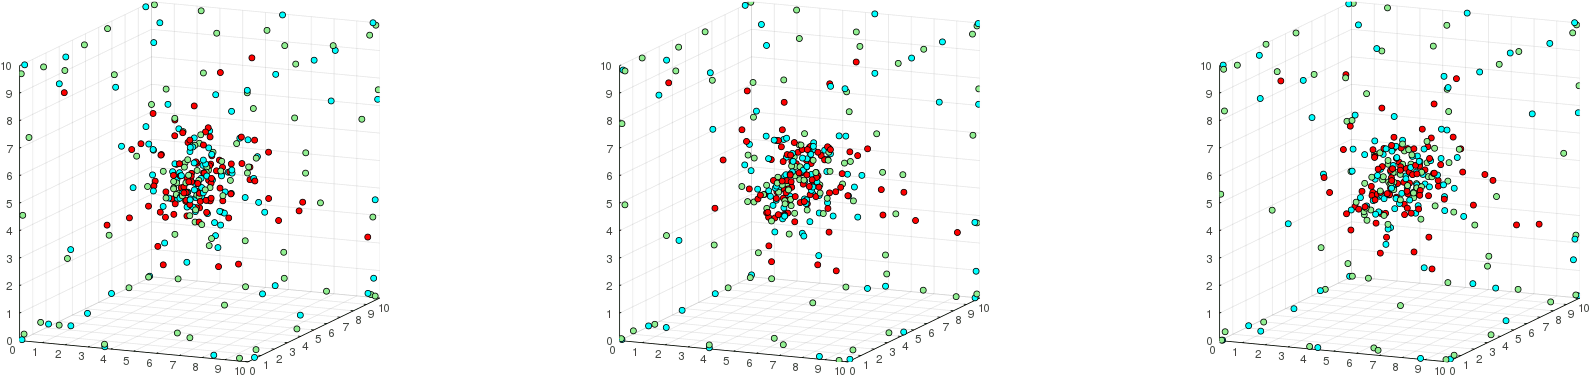
\includegraphics[width=\textwidth]{images/spritesheet3d.png}
\caption{Un esempio di simulazione in 3D di un sistema non periodico, vincolato, composto da 300 particelle di 3 tipologie diverse evidenziate dai colori.}
\label{sprite3d}
\end{figure}
\section*{Panoramica}
Questo progetto conclusivo relativo al corso di calcolo parallelo e distribuito tenuto dal prof. Alberto Paoluzzi all'università di Roma Tre, ha come principale obiettivo l'applicazione delle tecniche di calcolo parallelo su \textbf{G}raphics \textbf{P}rocessing \textbf{U}nit e nello specifico GPU \textbf{nVidia}, sfruttando il toolkit \textbf{CUDA} \cite{CUDA}. Inoltre, per poter avere un termine di paragone valido delle prestazioni ottenute, è stata realizzata anche la parallelizzazione su CPU con multi-thread, nonché l'esecuzione seriale.

L'intero progetto si basa su un lavoro precedente di Emily Crabb \cite{crabb} sulla simulazione delle dinamiche molecolari, nel quale sono state esplorate diverse tecniche di calcolo parallelo ed anche distribuito ad eccezione della versione su GPU, lasciata incompleta. Da qui in poi sarà il "progetto originale". In parole povere si tratta di calcolare posizione, velocità ed accelerazione di un certo numero di particelle ad ogni istante di tempo per un certo numero di istanti di tempo. L'algoritmo implementato è noto come \textbf{Velocity Verlet} \cite{verlet} e consiste nell'applicazione di tre formule, per ogni particella, nota a priori la forza agente su quella particella. 

Il linguaggio di programmazione utilizzato è il \textbf{Julia} \cite{julia}, che recentemente sta riscuotendo un crescente successo nell'ambito della computazione scientifica e che al contempo possiede caratteristiche in grado di permettergli un impiego anche nella realizzazione di software commerciali, combinando un elevato potere espressivo in stile Python, con prestazioni paragonabili al C/C++ (se opportunamente ottimizzato) risolvendo quindi il \emph{two language problem}.

Un aspetto, spesso sottovalutato, del calcolo numerico su grandi quantità di dati, è la visualizzazione dei risultati, non solo per poter avere una migliore comprensione degli stessi ma anche per individuare molto più facilmente eventuali anomalie o imprecisioni inaccettabili. Il progetto originale visualizza il sistema soltanto nello stato iniziale ed in quello finale, mostrando le posizioni delle particelle nello spazio. Ciò potrebbe non permettere di individuare, ad esempio, delle traiettorie palesemente errate.\\
In questo progetto si è realizzato un semplice sistema di animazione ``a posteriori'' (nel senso che l'animazione viene generata dopo che il calcolo delle posizioni in ogni istante di tempo è stato completato), in grado di generare una \texttt{gif} che mostra l'evoluzione del sistema in tempo reale a \texttt{30fps}. In questo modo è stato possibile notare subito che qualcosa non andava come avrebbe dovuto, nella versione iniziale del codice.

%%%%%%%%%%%%%%%%%%% SERIALE %%%%%%%%%%%%%%%%%%%%%%%%%%%%%%%%%%
\section{Revisione e riscrittura della versione Seriale}
Sono trascorsi più di due anni dal lavoro originale che hanno portato diversi cambiamenti sia nelle possibilità offerte da Julia che in quelle offerte da nVidia per quanto riguarda CUDA. 
Per questi motivi si è svolta una revisione completa del codice seriale e ciò ha permesso di identificare alcuni problemi di gestione dei salvataggi, facilitato una comprensione dell'algoritmo generale e quindi di riformulare alcuni concetti di base che hanno comportato modifiche più o meno sostanziali a seconda del caso.

Nel progetto originale si definisce la possibilità di simulare sistemi finiti o infiniti, inoltre, un sistema finito può essere periodico oppure no. Dopo aver cercato maggiori informazioni sulle condizioni di periodicità di un sistema, comunemente utilizzate in questo campo, è stata presa la decisione di riorganizzare l'idea di base, rimuovendo il concetto di sistema infinito pur mantenendo la stessa possibilità di simularlo ed aggiungendo un'ulteriore opzione. In questa revisione, ogni sistema è considerato finito per i limiti fisici imposti da un calcolatore. Un sistema finito può essere periodico o non periodico. Ogni sistema, periodico o no, a sua volta, può essere vincolato o non vincolato. Qualora si volesse modellare un sistema teoricamente infinito, basta scegliere un sistema non periodico senza vincoli. In figura \ref{treesys} viene mostrata la nuova classificazione dei modelli rappresentabili.

\begin{figure}[ht]
\centering
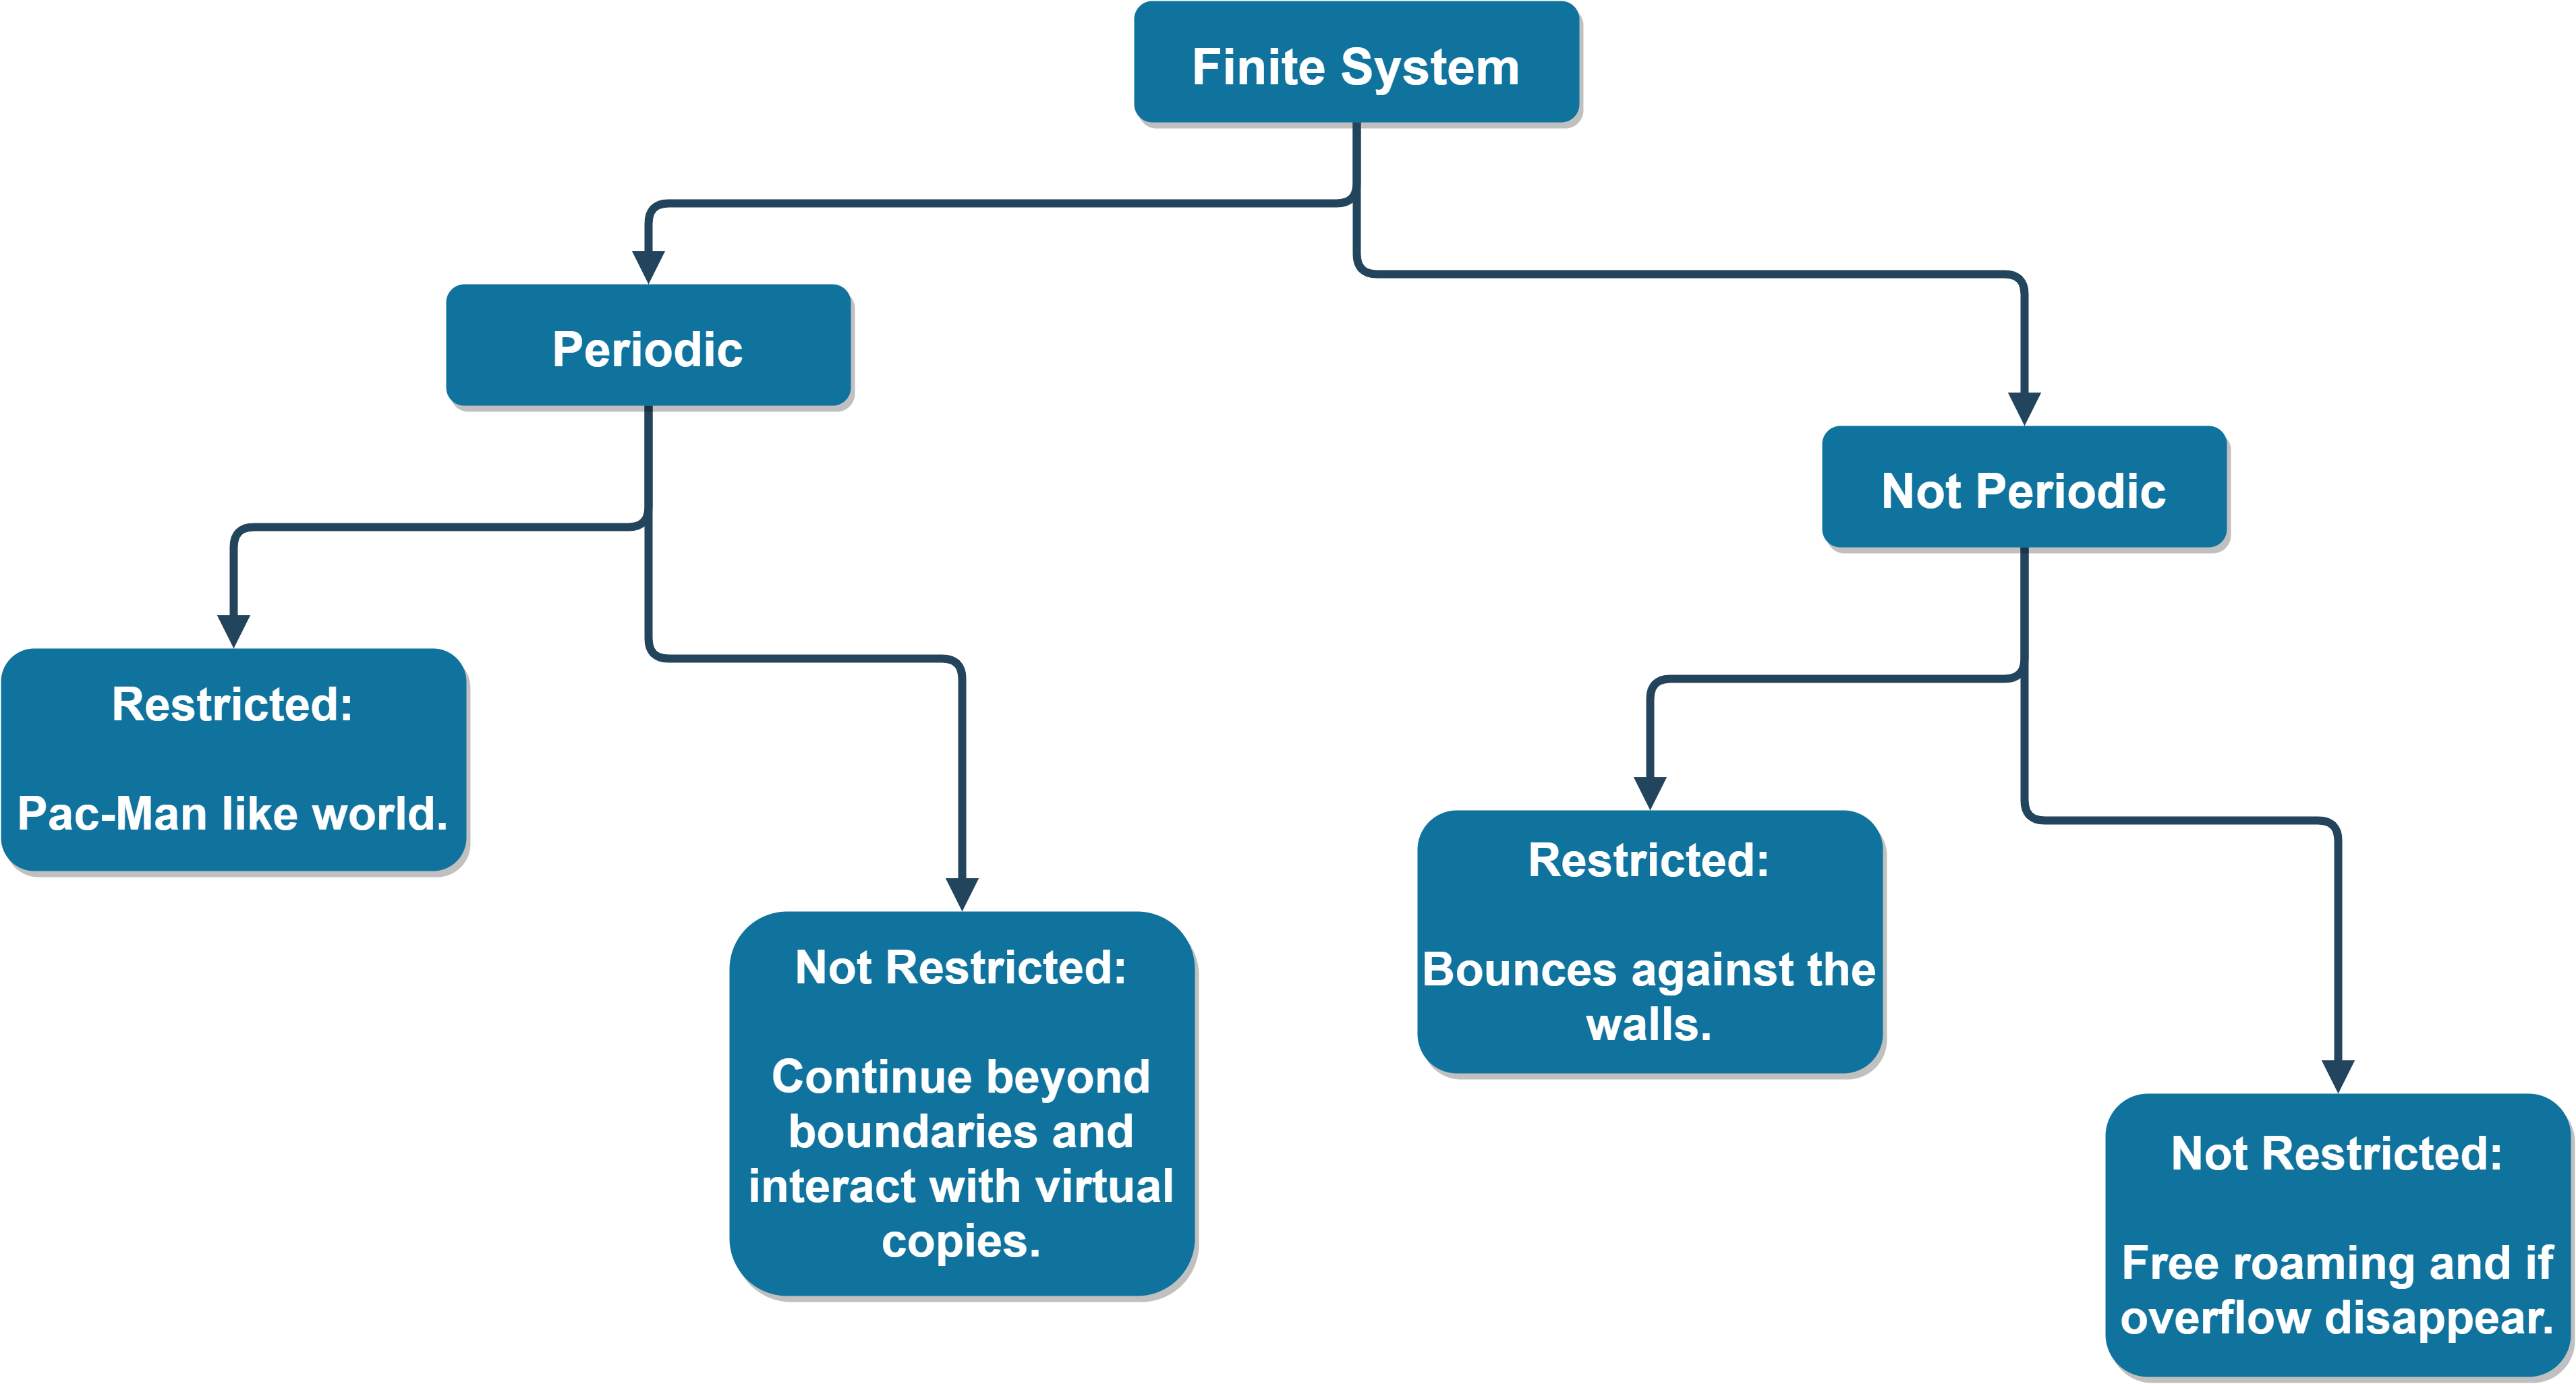
\includegraphics[width=\textwidth]{images/Treediag.png}
\caption{Tipologie di sistemi modellabili. Per un computer, un sistema infinito può essere approssimato con un sistema finito, non periodico e senza restrizioni.}
\label{treesys}
\end{figure}

Come precedentemente accennato, questa diversa classificazione introduce un nuovo tipo di sistema periodico senza restrizioni che prima non veniva considerato: In questo nuovo caso una particella che supera il confine è libera di continuare, interagendo con delle copie virtuali delle particelle presenti all'interno del confine iniziale.

Durante le prime prove di simulazione con animazione, si poteva osservare uno strano effetto che faceva muovere improvvisamente le particelle ad altissime velocità su traiettorie fra loro quasi parallele, contrariamente a quanto sarebbe dovuto accadere. Questo era dovuto ad un errore nel calcolo della forza, che consisteva nell'applicare la formula a ciascuna componente vettoriale piuttosto che alla distanza stessa.
\begin{figure}[ht]
\centering
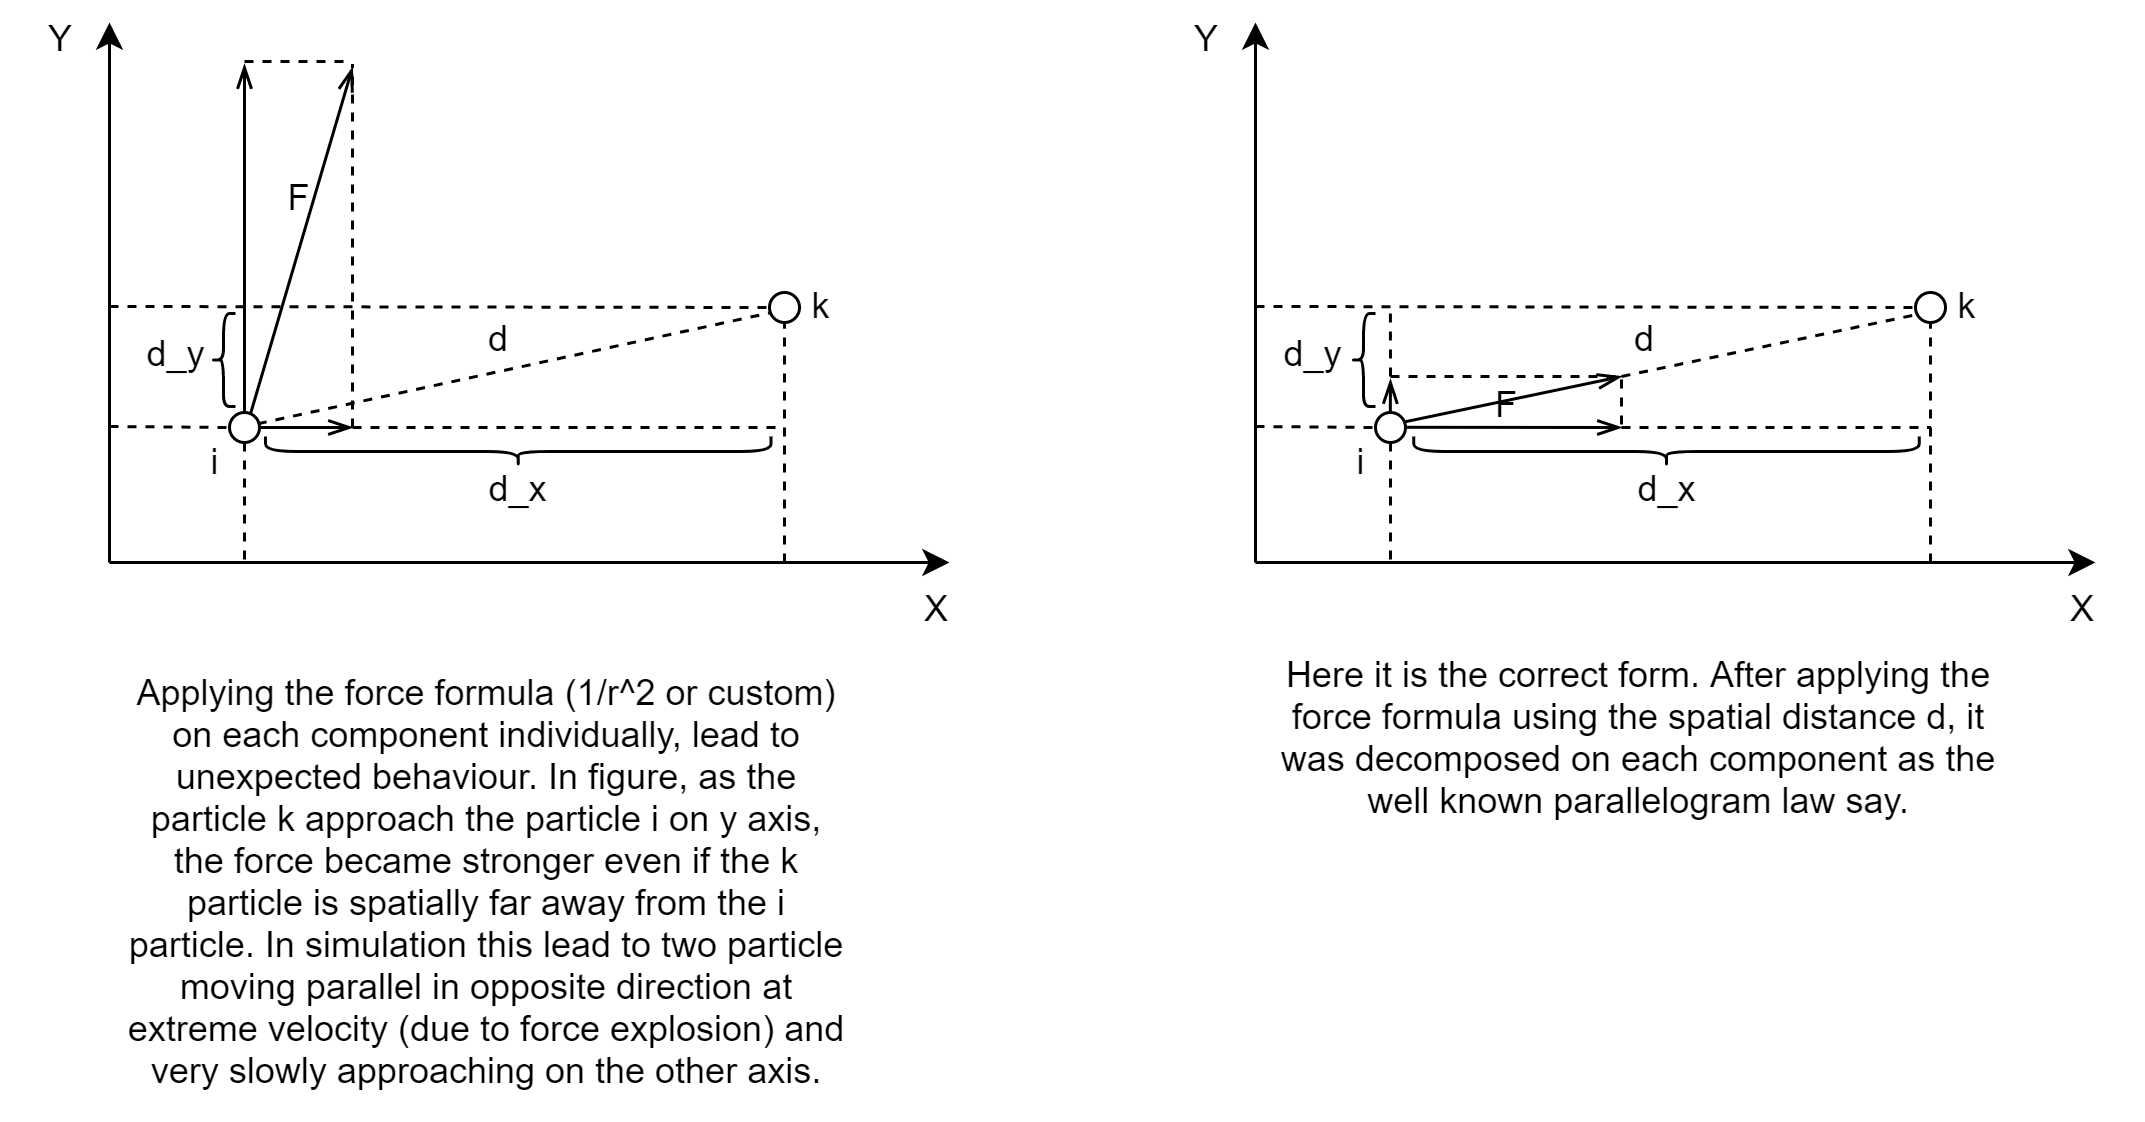
\includegraphics[width=\textwidth]{images/ForceError.png}
\caption{L'errore nel calcolo della forza. A sinistra, la particella k pur trovandosi distante dalla particella i esercita una forza sempre più forte sulla sua componente y, generando una forza F quasi parallela.}
\label{forcerror}
\end{figure}
Da notare che sarebbe stato difficile da rilevare basandosi solo sul risultato numerico finale, l'algoritmo infatti prevede la scomposizione di ogni operazione sulle componenti dimensionali di ciascun asse (i.e. x, y, z, nello spazio tridimensionale oppure x, y in quello bidimensionale).\\
Di seguito viene riportata la porzione di codice che genera il problema:
\begin{verbatim}
for j = 1:dim # For each dimension
...
   dist = abs(pos[i,j] - pos[k,j])
...    
   force[i,j] += int_strength / dist^2 # 1/r^2 interaction
end
\end{verbatim}
Riferito alle generiche particelle \texttt{i} e \texttt{k}.

Sebbene si possa contare sul sistema automatico di inferenza di tipi nonché sul \emph{multiple dispatch} di Julia che produce diverse versioni (metodi) associati ad una funzione specializzati in parametri con tipi diversi, si è scelto di specificare il principale tipo numerico per i calcoli come \texttt{Float32} in previsione del confronto con la versione CUDA in cui è consigliato l'uso di questo tipo di dato per cui è ottimizzata, oltre al fatto che consuma meno memoria in caso di grandi allocazioni per matrici e vettori.  

Il sistema di salvataggio su disco dei dati generati per una eventuale ripresa della simulazione è stato rivisto, in una forma più semplice che sfrutta le primitive \texttt{serialize} e \texttt{deserialize} messe a disposizione dal package \texttt{Serialization} della libreria standard di Julia. In questo modo tutto ciò che serve viene salvato in un unico file, che termina con \texttt{\_data}, binario, riducendo il numero dei file generati da un salvataggio al prezzo di non consentirne più la modifica manuale. 

In breve, ogni caratteristica del software originale è stata mantenuta e ne sono state introdotte di nuove.
Alcune ulteriori modifiche e novità introdotte:

\begin{enumerate}
    \item Costante d'attrito per dissipare la forza progressivamente;
    \item Costante di rimbalzo per urti anelastici con le pareti;
    \item Utilizzato il segno della distanza per direzionare la forza;
    \item La matrice delle forze veniva riallocata ad ogni iterazione;
    \item Limite per la distanza minima;
    \item Variabili allocate fuori dai cicli;
    \item Macro \texttt{@fastmath} nelle espressioni numeriche complesse per prestazioni migliori.
\end{enumerate}

%%%%%%%%%%%%%%%%%%%%%%%%% CUDA %%%%%%%%%%%%%%%%%%%%%%%%%%%%%%%
\section{Scrittura della versione Multi Thread con CUDA}
L'architettura CUDA viene resa accessibile in Julia dai package CuArrays, CUDAnative e CUDAdrv \cite{CUDAJL}. Per semplici operazioni di algebra lineare come il calcolo matriciale, esistono già predefinite delle funzioni, omologhe a quelle già esistenti nella libreria standard, che operano sulla struttura dati fondamentale: il \texttt{CuArray}, corrispettivo del classico Array ma memorizzato in VRAM. Queste funzioni predefinite, nello specifico gli operatori di broadcasting, se combinate permettono di realizzare operazioni più complesse come se si usassero i classici Array generando automaticamente codice macchina già ottimizzato. Tuttavia in alcuni casi particolari possono non risultare sufficienti e quindi si rende necessario creare delle funzioni specializzate in grado di essere eseguite direttamente dalla GPU sfruttandone capacità di parallelizzazione in modo più fine. Queste funzioni sono dette kernel function ed in questo progetto ne sono state realizzate due, sovrapponibili alle funzioni \texttt{find\_forces!} e \texttt{step\_update!}, che implementano la medesima logica.

Nell'immagine in figura \ref{cudasplit} viene mostrato concettualmente come viene diviso il lavoro fra i threads disponibili su una GPU. Nell'architettura CUDA è necessario specificare i threads per blocco che variano a seconda del sistema e delle risorse disponibili. 
\begin{figure}[ht]
\centering
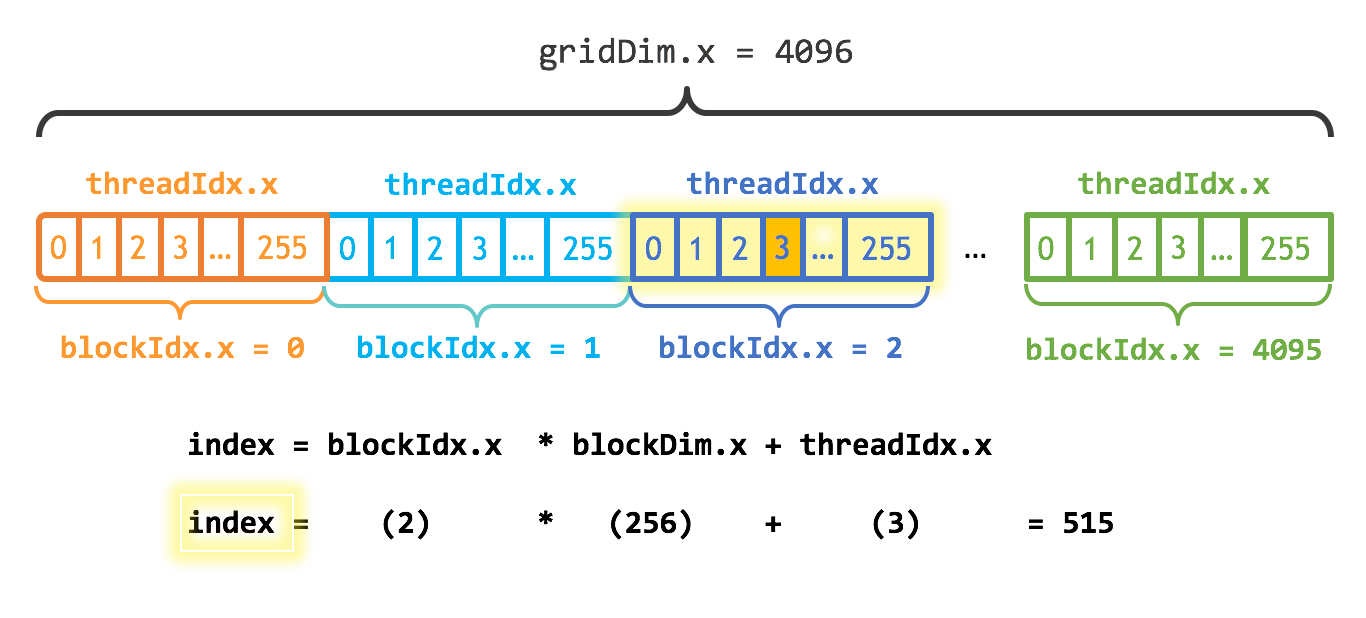
\includegraphics[width=\textwidth]{images/cudaparal.png}
\caption{Suddivisione del lavoro in blocchi con 256 threads}
\label{cudasplit}
\end{figure}
Facendo riferimento all'immagine, si supponga ad esempio di avere $n$ particelle da simulare e 256 threads per blocco, dividendo $n/256$ si ottengono il numero di blocchi totali ciascuno con 256 thread paralleli. Volendo mappare l'indice di ciascuna particella da $1$ a $n$ su ciascun thread si ottiene la formula in figura che poi è stata implementata nel codice sorgente:
\begin{verbatim}
function find_forces!(forces, pos, vel, acc, ...)
    
    # Parametri per kernel function CUDA
    index = (blockIdx().x - 1) * blockDim().x + threadIdx().x
    stride = blockDim().x * gridDim().x
...
    # Per ogni particella i
    @inbounds for i in index:stride:part_num        
        # Calcola la massa di i
        mass1 = mass_parts[part_types[i]] 
        # Per ogni altra particella k diversa da i
        for k in 1:part_num
...
\end{verbatim}

In questo caso si noti che ogni thread deve comunque considerare tutte le altre particelle serialmente, accumulandone il risultato per ciascuna componente della forza. Perciò l'accesso concorrente (in scrittura) alla matrice delle forze rende impossibile parallelizzare il loop interno a patto di non usare una struttura dati ausiliaria (un tensore tridimensionale) sulla quale eseguire una riduzione in un secondo tempo ed utilizzando quindi due funzioni kernel. Ad ogni modo l'esecuzione parallela di loop seriali comporta comunque delle buone prestazioni che saranno evidenziate più avanti.

%%%%%%%%%%%%%%%%%% CPU MultiThreads %%%%%%%%%%%%%%%%%%%%%%%%%%%%%
\section{Revisione e riscrittura della versione CPU multi-thread}
Contrariamente alla versione CUDA in cui il calcolo da effettuare viene suddiviso in blocchi, ciascuno con un certo numero di threads, nel caso della CPU si è seguito il codice originale che utilizza la macro \texttt{@threads} per avviare un numero di processi paralleli pari al numero di particelle.
Viene riportato il codice sorgente della funzione \texttt{find\_forces!} in cui si può notare che le variabili vengono allocate all'interno del ciclo \texttt{for} che avvia ciascun thread.
\begin{verbatim}
...
# Per ogni particella i
@threads for i in 1:part_num
        
    # Alloca variabili per il thread corrente
    mass1 = .0f0 # Massa particella i
    mass2 = .0f0 # Massa particella k
    int_strength = .0f0 # Forza di interazione
    distance = .0f0 # Distanza fra i e k        
    force_strength = .0f0 # Forza esercitata da k su i

    @inbounds begin
        # Calcola la massa di i
        mass1 = mass_parts[part_types[i]]
        # Per ogni altra particella k diversa da i
        for k in 1:part_num
...
\end{verbatim}

%%%%%%%% BENCHMARK %%%%%%%%%%%%%%
\section{Benchmark}
Le prestazioni sono state misurate sfruttando il package BenchmarkTools, su due calcolatori, uno un po' datato, con processore \texttt{Intel Core i7-950 @ 3.06 GHz, 4 Core, 8 Thread} e scheda grafica \texttt{GTX 970}, ed uno di nuova generazione, con processore \texttt{Intel Core i7-9750H @ 2.60 GHz, 6 Core, 12 Thread}, dotato di scheda grafica \texttt{RTX 2060}, estendendo i test del progetto originale fino a 1500 particelle e mantenendo gli stessi parametri di simulazione (dimensione del box, variabile dt, periodicità, ecc..).
Si tenga presente che aspettarsi risultati esattamente uguali è poco ragionevole, perché: 
\begin{enumerate}
    \item La macchina usata per i test originali è differente; 
    \item Il nuovo codice contiene alcune modifiche sostanziali e correzioni;
    \item L'utilizzo della macro \texttt{@sync} in entrambe le versioni parallele garantisce che vengano misurate correttamente le prestazioni, cosa che \textbf{non veniva fatta nel benchmark originale}. In questo modo il tempo misurato fa riferimento all'effettivo termine di tutti i threads;
    \item La versione di Julia è differente e quindi potenzialmente anche il codice macchina generato dal compilatore.
\end{enumerate}

In figura \ref{victor} i risultati del benchmark sul pc più "datato". Si può notare l'andamento della versione CUDA che scala in maniera quasi lineare rispetto al numero di particelle. La piccola singolarità riscontrabile a 500 particelle, probabilmente non è dovuta al caso e test ripetuti evidenziano lo stesso comportamento, forse da imputare ad una leggermente miglior ottimizzazione del codice multi thread da parte del compilatore JIT oppure ad un piccolo collo di bottiglia tra CPU e GPU.

\begin{figure}[ht]
\centering
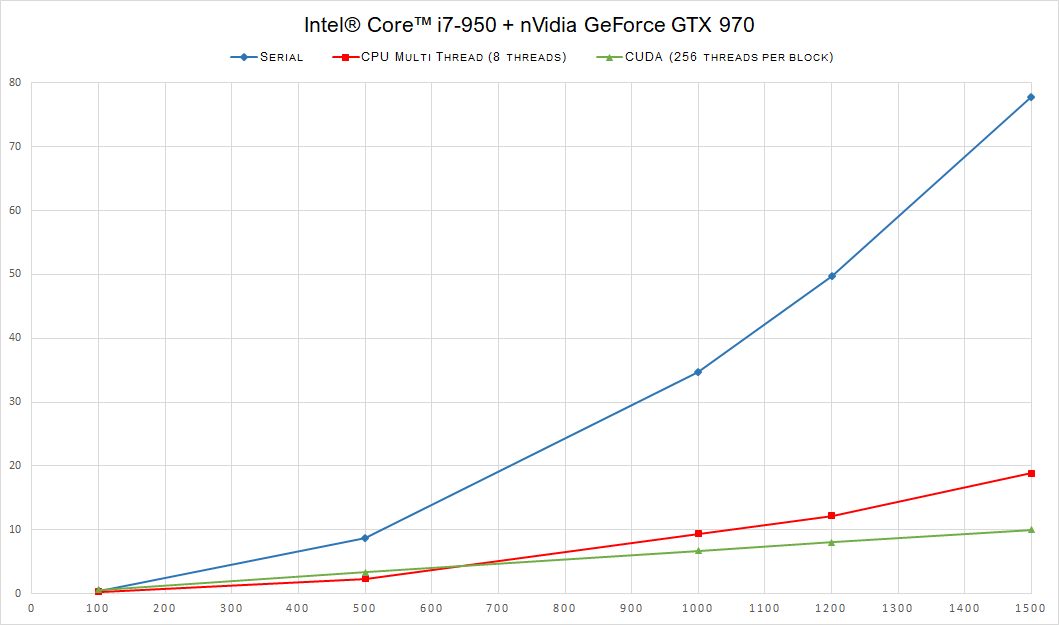
\includegraphics[width=\textwidth]{images/victorBenchmark.png}
\caption{Asse X: Numero di particelle, Asse y: Durata media del calcolo}
\label{victor}
\end{figure}

In figura \ref{romeo} i risultati del PC con hardware di nuova generazione. Appare evidente come lo stesso codice Julia produca codice macchina ottimizzato che scala coerentemente con le maggiori risorse a disposizione. Da tenere presente che sia nella configurazione precedente che in questa si è sfruttato l'\textbf{hyperthreading} consentendo al processore di usare tutti i \emph{core logici}. In questo caso i 12 Threads hanno certamente ridotto il divario con la versione CUDA pur restando quest'ultima la migliore in ogni caso.
Il numero di threads per blocco è stato scelto, in entrambe i casi, in modo da essere il massimo assegnabile con l'intento di misurare le prestazioni della GPU al massimo del parallelismo offerto, nonostante qui non siano stati riportati i risultati per valori inferiori, dalle numerose prove empiriche condotte, ci si può aspettare un tempo medio leggermente maggiore. 
\begin{figure}[ht]
\centering
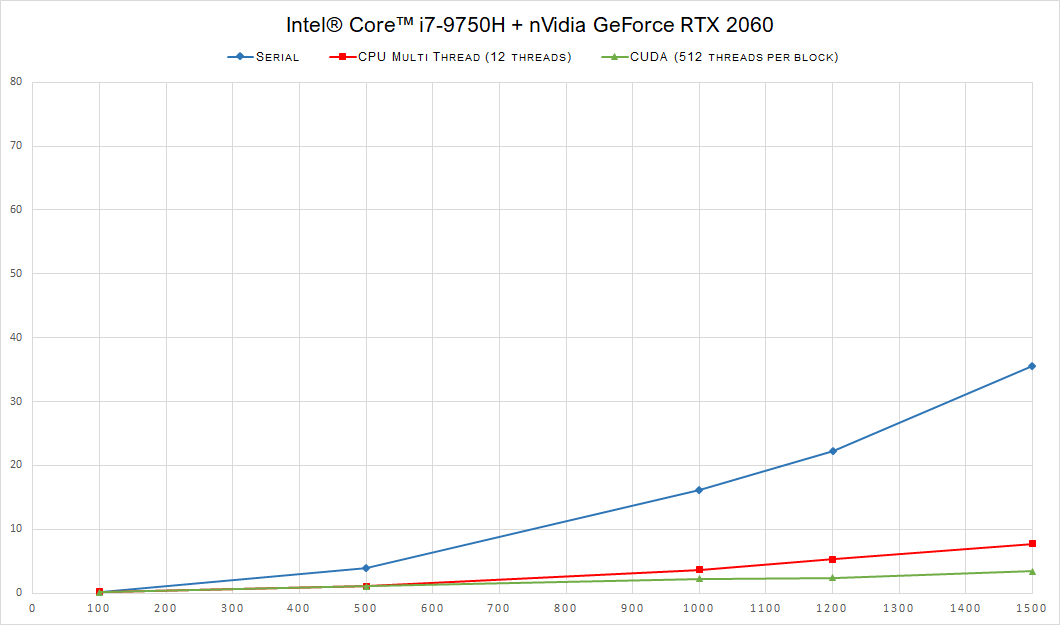
\includegraphics[width=\textwidth]{images/romeoBenchmark.png}
\caption{Asse X: Numero di particelle, Asse y: Durata media del calcolo}
\label{romeo}
\end{figure}

%%%%%%%%%%% VISUALIZZAZIONE %%%%%%%%%%%%%%
\section{Visualizzazione con animazioni}
Come accennato all'inizio, una parte secondaria di questo progetto riguarda la visualizzazione del moto delle particelle che non era stata affrontata nel lavoro originale, maggiormente concentrato sul confronto delle tecniche di calcolo parallelo. 
\begin{figure}[ht]
\centering
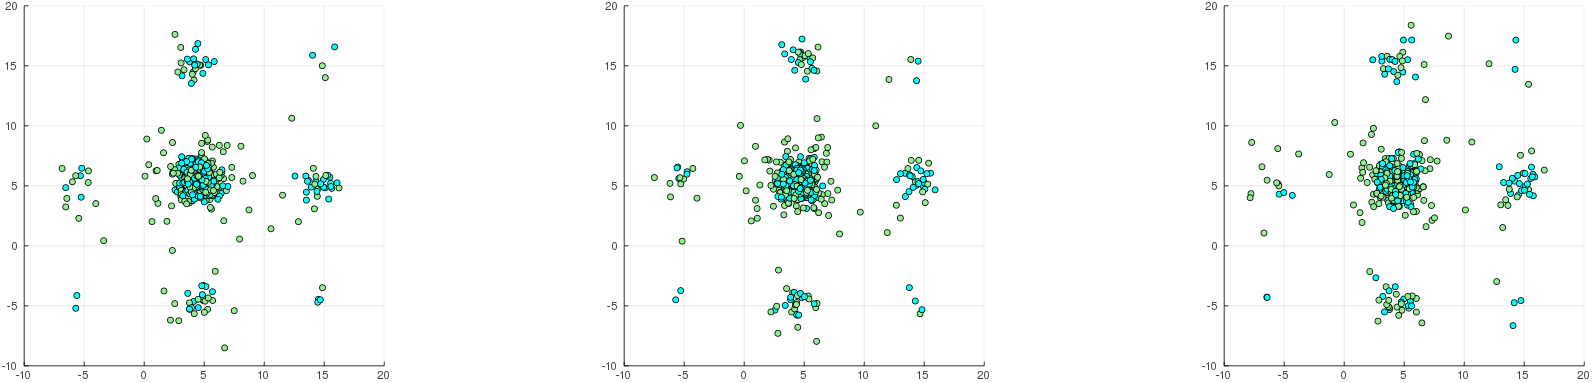
\includegraphics[width=\textwidth]{images/spritesheet2d.png}
\caption{Esempio del nuovo tipo di sistema periodico, senza restrizioni in 2D.}
\label{sprite2d}
\end{figure}
Con l'intenzione di realizzare un'animazione sufficiente a dare un'idea chiara dell'evoluzione del sistema, si è utilizzato il package Plots. Questo package, orientato alla visualizzazione generica di grafici, offre la possibilità di animare un grafico generandone uno per ciascun frame con dati diversi. Questa caratteristica, combinata con il più classico \emph{scatter plot} ha rappresentato un'idea semplice ma funzionale per realizzare delle animazioni del moto delle particelle sia in 3D che in 2D. Raffinando ancora un po' questo metodo si è scelto di colorare ciascun tipo di particella in modo da rendere chiaro il tipo di interazione atteso.
Inoltre, considerando un framerate standard di 30fps, è stato calcolato il $\delta$t opportuno per produrre un'animazione a velocità reale.
Alcuni esempi di animazioni generate con questo metodo sono disponibili sul repository pubblico di questo progetto \cite{myself}.

%%%%%%% CONCLUSIONI %%%%%%%%%%%%%
\section*{Conclusioni e sviluppi futuri}
L'algoritmo in generale è basato su due funzioni: una per calcolare le forze ed una che aggiorna le posizioni delle particelle. Queste due funzioni vengono eseguite ripetutamente un gran numero di volte. Nel corso della riscrittura sono stati trovati alcuni bug e migliorate alcune parti tuttavia questo non vuol dire che le scelte fatte siano tutte giuste ed anzi in alcuni casi il dubbio è rimasto. Alcune idee sono state scartate perché richiedevano un cambiamento radicale della logica del programma, come ad esempio utilizzare una singola struttura dati per memorizzare posizioni velocità ed accelerazioni (tensore tridimensionale). Ridurre il numero di parametri passati ed evitare ridondanze faciliterebbe notevolmente la scrittura di codice parallelizzato.

Il sistema di salvataggi è stato certamente semplificato, tuttavia il prezzo di non poter manualmente modificare i dati salvati potrebbe essere eccessivo in certi casi, ad esempio come una primitiva interfaccia utente che permetta l'inserimento manuale dei parametri di simulazione senza dover ri-dichiarare costanti nel codice.

La versione CUDA potrebbe essere migliorata scrivendo dividendo le funzioni kernel in funzioni più piccole che portano a risultati parziali, combinando tutto con operazioni di broadcast dove possibile, infatti l'uso di tali operatori non è consentito all'interno di kernel dal momento che essi stessi sono implementati come kernel e può esserci un solo kernel in esecuzione in un certo momento sulla GPU.

Per quanto riguarda le versioni \emph{CPU Multi Thread} e \emph{Seriale} si potrebbe sfruttare l'utilizzo maggiore di operatori di broadcast per aggiornare le dimensioni eliminando i \texttt{for} ripetuti per il calcolo della distanza  ed oltre a questo indagare su possibili utilizzi degli StaticArray.


%\flushright{\textit{``We adore chaos because we love to produce order.''} -- \emph{M.C. Escher}}

\printbibliography

\end{document}